\chapter{Konzeption}

\section{Vorangehende Arbeit}
Diese Arbeit baut auf dem Design des Youtubers \glqq Matthew Perks\grqq{} auf. Sein Ziel war es eine Beleuchtung zu schaffe, die in den dunklen Monaten die Stimmung hebt und damit die Produktivität des Nutzers fördert \cite{Perks20}. Vermutlich aus Kosten und Komplexitätsgründen wurde auf die Variabilität der Farbtemperatur und den veränderlichen Einfallswinkel verzichtet.

Als Lichtquelle nutzt dieses Design eine COB-LED mit 500w Leistung, einem hohen CSI-Index von 95 und einem Kelvinwert von 5600, was die Beleuchtung durch Morgensonne realistisch nachahmt. Zur Kühlung dieser Led wird eine System auf Basis einer Wasserkühlung für einen Computer verwendet. Um die Lichtstrahlen der LED parallel auszurichten, baute er mithilfe von reflektierender Folie eine Satellitenschüssel zu einem Parabolspiegel um. Die letzte ausschlaggebende Komponente ist ein dünnes, einem Fenster ähnliches transparentes Behältnis das mit Seifenwasser befüllt ist. Dies dient zur Simulation der Atmosphäre, da hier das Licht durch die kleinen Partikel ebenso in einen diffusen bläulichen und einen direkten gelblich Anteil aufgespalten wird.

\begin{figure}[H]
	\centering
	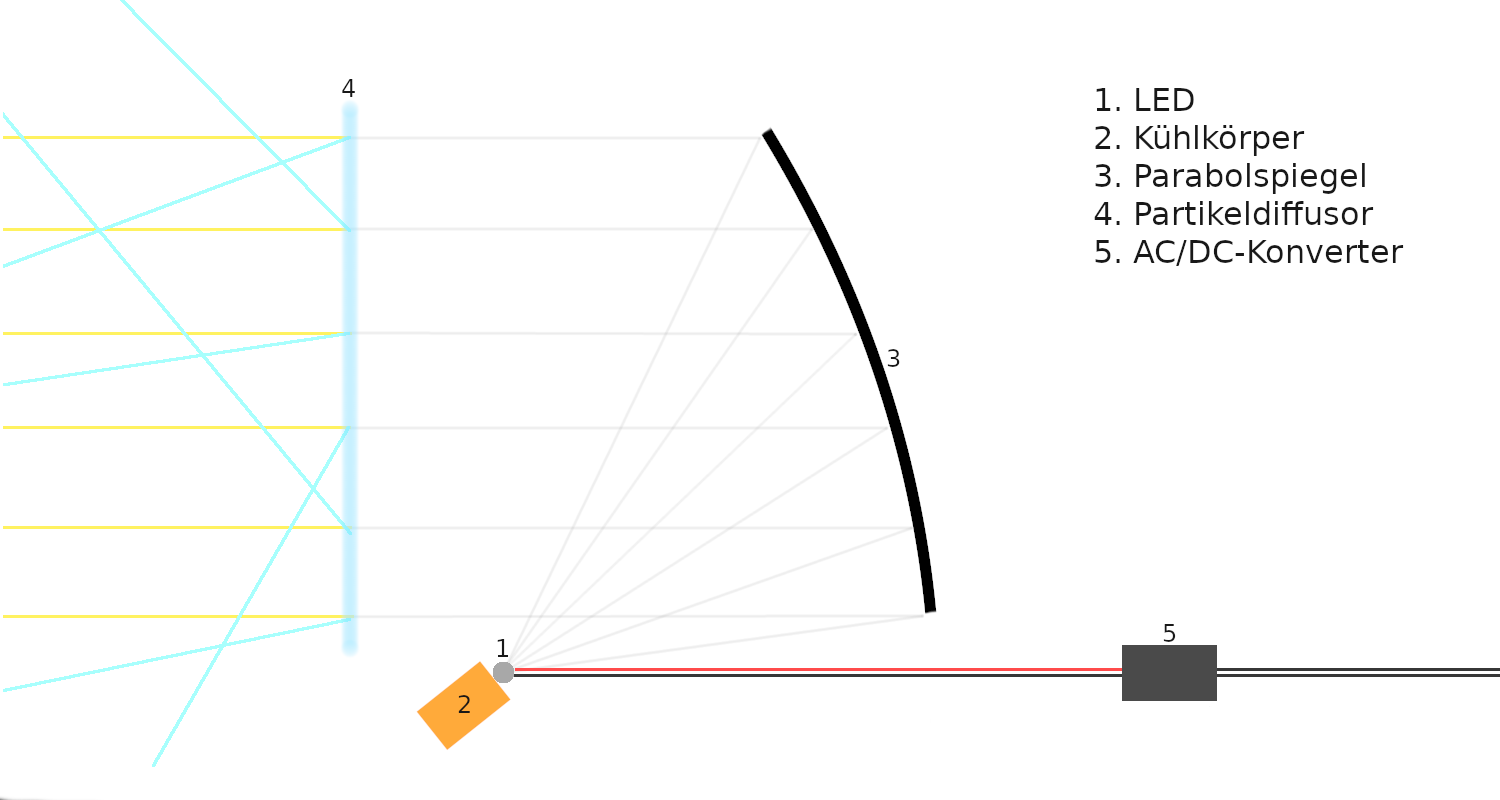
\includegraphics[width=0.95\textwidth]{resources/own_content/sun-design}
	\caption{Funktionsprinzip der Beleuchtung \cite{LePr}}
	\label{img:funktions_prinzip}
\end{figure}

\section{Hardware Konzeption}
Das Design braucht noch einige elektronische Komponenten um automatisiert betrieben zu werden. So braucht es zumindest einen Mikrocontroller um Daten verarbeiten zu können. Dieser Mikrocontroller braucht zudem einen Lichtsensor um auf die Beleuchtungssituation reagieren zu können. Zudem braucht es einen Weg, die Einstellungen einzusehen und manipulieren zu können. 

Da Mikrocontroller in der Regel nicht direkt mit der hohen benötigten Leistung der LED arbeiten können, wurde eine Schnittstelle zwischen Mikrocontroller und der Stromzufuhr der LED benötigt. Aus Gründen der Komplexität wird hier ein Relais vorgesehen. Ein Dimmer würde einen fließenden Übergang zwischen natürlichem um künstlichem Licht ermöglichen. Doch aufgrund mangelnder elektrotechnischer Erfahrung wird in dieser Arbeit auf die einfachere Art der binären Schaltung gesetzt.

Abschließend brauchen diese beiden weiteren Komponenten auch eine Stromversorgung. Zwar nutzt das grundlegende Design schon ein Leistungsfähiges Netzteil, dieses kann aber wegen der unpassenden Spannung nicht direkt für den Mikrocontroller und das Relais genutzt werden. Denn im Gegensatz zu der LED nutzen diese Komponente in der Regel eine sehr viel niedrigere Arbeitsspannung. Aus diesem Grund ist mindestens ein Buck-Konverter für die Wandlung des Stroms von Nöten. Hierdurch können alle Komponenten durch ein einzige Stromquelle versorgt werden.

\section{Software Konzeption}

\subsection{Grundlegende Architekturen}
Da ein Mikrocontroller in der Regel nicht mit Hardware zur Anzeige oder Intuitiven Eingabemöglichkeiten ausgestattet ist, muss diese anderweitig bereit gestellt werden. Glücklicherweise erfreuen sich Smartphones weiter Verbreitung und stellen mit ihren Displays ideale Kandidaten für das Interface dieses Anwendungszweck dar. Aufgrund des hohen Marktanteils wurde Android als Zielplattform gewählt.

Die Wahl der Software für den Mikrocontroller viel auf Micropython. Diese Wahl wurde aufgrund des Hohen Abstraktionsgrades dieser Sprache gewählt, wodurch eine potentiell schnelle Implementierung der Funktionen ermöglicht werden sollte.

\subsection{Kommunikation der Komponenten}
Die Kommunikation zwischen diesen beiden Plattformen sollte drahtlos per TCP über Wifi passieren. Diese Wahl wurde unter der Annahme getroffen, das eine solche Lampe nur stationär in der Wohnung des Besitzer verwendet wird, wo schon ein Wlan aufgespannt wurde. Im Gegensatz zu Bluetooth hat dies den Vorteil, dass nicht jedes mal erst ein Pairing-Prozess angestoßen werden muss um die Beleuchtung anpassen zu können und davon ausgegangen werden kann, dass zuhause mobile Endgeräte sowieso schon hiermit verbunden sind.

\subsection{Nutzerinterface}
Damit die Lampe möglichst intuitiv zu bedienen ist und alle Funktionen nicht mehr als einen Klick benötigen, sollten alle Features von einem zusammenhängendem Panel erreichbar sein. Zudem sollten die meist genutzten Funktionen in der Nähe des Daumens verortet sein, um sie noch einfacher erreichbar zu machen. Es kann davon ausgegangen werden, dass ein durchschnittlicher Mensch nicht mit Einheiten zur Messung der Lichtintensität und schon gar nicht mit ihrer Interpretation vertraut ist. Aus diesem Grund wurde die Visualisierung der Messdaten des Vortages in Form von Graphen eingeplant, um dem Nutzer einen Orientierungspunkt für Konfigurationen zu bieten. Dieser sollte die Zeit in der x-Achse und die Lichtintensität an der y-Achse widerspiegeln. Dies legte die Wahl nahe, Schieberegler an den beiden Achsen zu platzieren um eine intuitive Einstellung der Zeit- und Lichtschwellenwerte für die Ein- und Ausschaltzeitpunkte zu ermöglichen. Zudem sollten alle momentanen Einstellungen in der Applikation ersichtliche sein. Dies soll durch eine entsprechende Farbgebung der Buttons und der entsprechenden Platzierung der Schieberegler möglich sein. Um eine Verbindung aufzubauen, muss ebenfalls eine Eingabe möglich sein. Da im vorherigen Abschnitt die Wahl der Kommunikation auf TCP fiel, sollte hier die IP-Adresse eingegeben werden. Da sich die IP wegen dem stationären Einsatzgebiets der Lampe nur, selten ändern sollte, wurde dieses Eingabefeld mit niedriger Priorität an den Oberen Rand des Panels geschoben. Das resultierende Design ist in der folgenden Abbildung ersichtlich.

\begin{figure}[H]
	\centering
	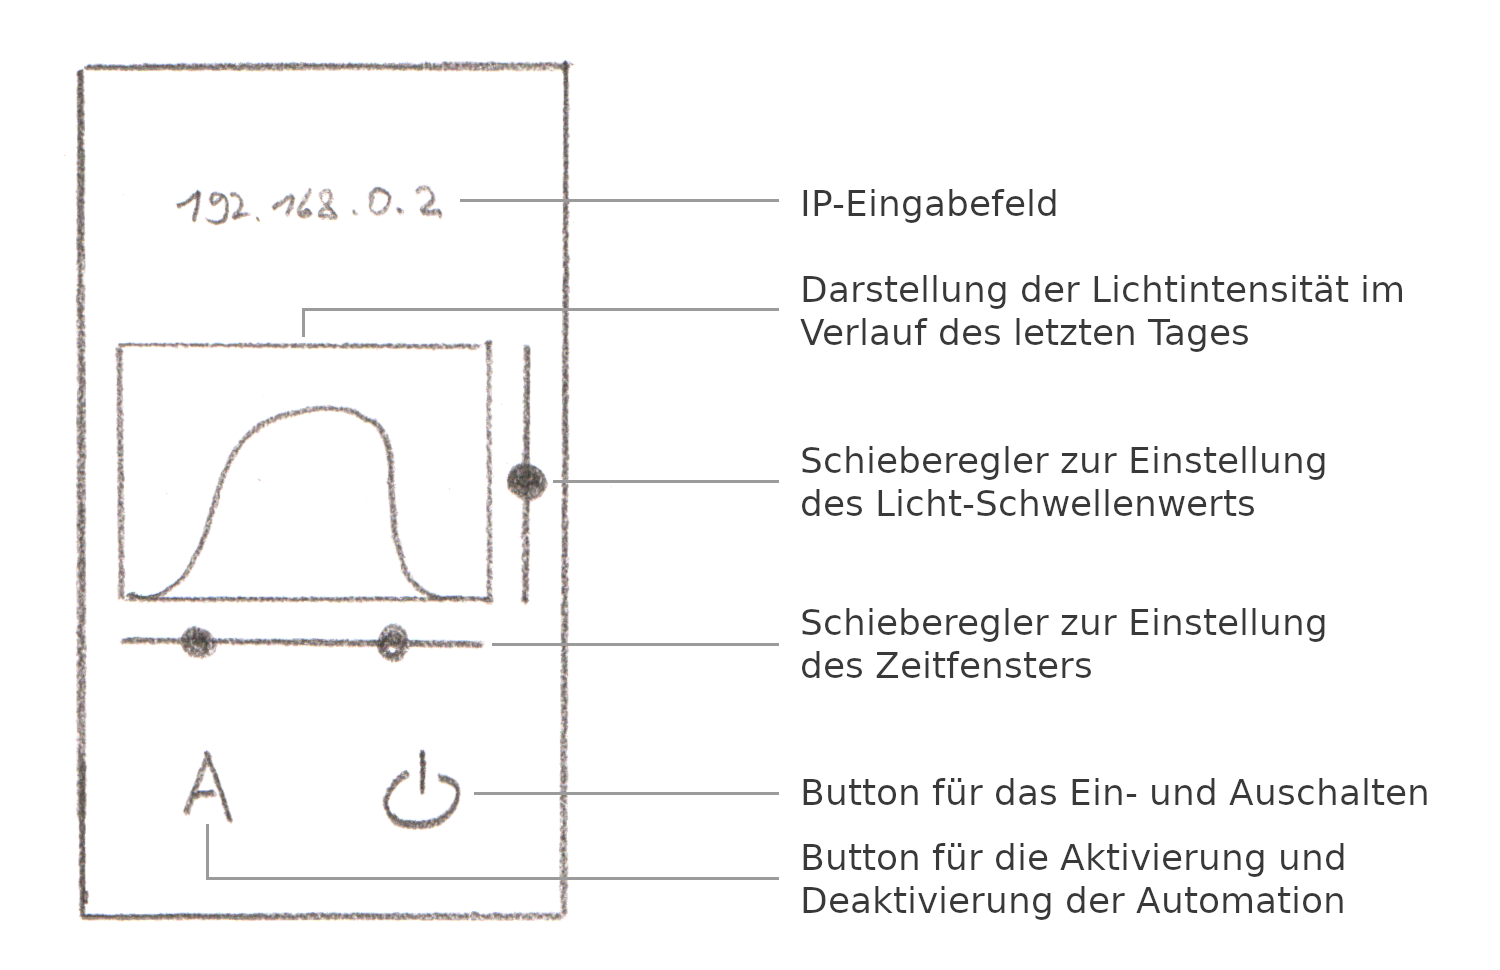
\includegraphics[width=0.95\textwidth]{resources/own_content/App_Design_Description}
	\caption{User Interface Entwurf \cite{LeIn}}
	\label{img:design_interface}
\end{figure}



